%%--------------------------------------------------
%----------------------------------------------------------------------
% options
\def\DisplayAuthors{0}
\def\DisplayFancyHeaders{0}
\def\DisplayAcknowledgements{0}

\documentclass[10pt,dvipdfm]{article}

%----------------------------------------------------------------------
%\usepackage{fullpage}
\usepackage[dvips]{graphicx}
\usepackage{amssymb}
\usepackage{amsmath}
\usepackage{verbatim}
\usepackage[usenames,dvipsnames]{color}

\setlength{\oddsidemargin}{-0.5truein}
\setlength{\evensidemargin}{-0.25truein}
\setlength{\textwidth}{7.3truein}
\setlength{\textheight}{10.0truein}
\setlength{\topmargin}{-1.0truein}
\setlength{\parskip}{3pt}


%----------------------------------------------------------------------
\title{Lab02 - Polynomials Using Linked Lists}
\date{}
%
\begin{document}
\maketitle

\vspace*{-2cm}

\noindent
%
\section{Assignment}
%
In mathematics, a polynomial is an expression constructed from variables (also known as indeterminates) and constants, 
using the operations of addition, subtraction, multiplication, and constant non-negative whole number exponents. 
For example, $x^2 - 4x + 7$ is a polynomial, but $x^2 - \frac{4}{x} + 7x^{3/2}$ is not, because its second term involves division by the 
variable x and also because its third term contains an exponent that is not a whole number.

Polynomials are one of the most important concepts in algebra and throughout mathematics and science. 
They are used to form polynomial equations, which encode a wide range of problems, from elementary word problems 
to complicated problems in the sciences; they are used to define polynomial functions, which appear in settings 
ranging from basic chemistry and physics to economics, and are used in calculus and numerical analysis to approximate 
other functions. Polynomials are used to construct polynomial rings, one of the most powerful concepts 
in algebra and algebraic geometry.

In this lab you will implement several functions to create and manipulate polynomials.
The terms of the polynomial will be stored in a singly linked list in decreasing order of the exponent values.

\begin{figure}[htbf]
\begin{center}
\begin{tabular}{c}
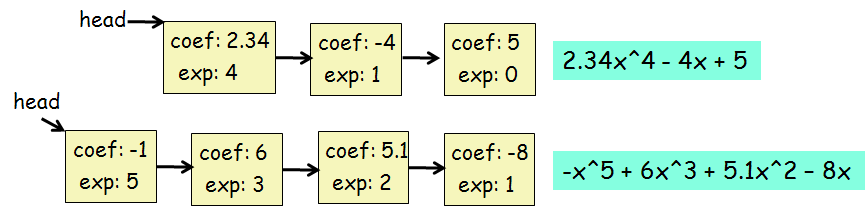
\includegraphics[width=5in]{FIG/1.png}
\end{tabular}
\caption{Representation of two polynomials using linked lists.}
\label{fig:poly} 
\end{center}
\end{figure}
%
Figure~\ref{fig:poly} depicts how P(x)=$2.34x^4 - 4x + 5$ and $-x^5 + 6x^3 + 5.1x^2 - 8x$ are 
represented by linked lists.
As seen, each term of the polynomial is represented by a PolyNode struct (defined in PolyNode.h), 
which consists of a coefficient and an exponent.
While a coefficient can be a real number, the exponent must be a natural number, i.e., an integer.
The terms of the polynomial are stored in decreasing order of their exponents in the linked list.

\subsection{Poly Creation and Operations}
%
A polynomial node is defined in PolyNode.h, and has the following structure:
\begin{verbatim}
struct PolyNode {
	double coef;             // Coefficient
	int exp;                 // Exponent
	struct PolyNode* next;   // Next polynomial node
}; //end-PolyNode
\end{verbatim}
%
Each node has a coefficient, which cannot be 0, and an exponent, which must be non-negative.

Polynomial functions are defined in Poly.h and implemened in Poly.cpp, and has the following prototypes:

\begin{verbatim}
PolyNode* CreatePoly(char* expr);
void DeletePoly(PolyNode* poly);
PolyNode* AddNode(PolyNode* head, double coef, int exp);
PolyNode* Add(PolyNode* poly1, PolyNode* poly2);
PolyNode* Subtract(PolyNode* poly1, PolyNode* poly2);
PolyNode* Multiply(PolyNode* poly1, PolyNode* poly2);
double Evaluate(PolyNode* poly, double x);
PolyNode* Derivative(PolyNode *poly);
void Plot(PolyNode* poly, int x1, int x2);
void Print(PolyNode* poly);
\end{verbatim}
%

A polynomial can be created by CreatePoly, which takes a string expression.
To implement this function, you are required to parse the given string
containing the polynomial expression into polynomial terms, 
and add each term to the constructed polynomial. 
The following are polynomial creation examples with expression strings:

\begin{verbatim}
PolyNode * poly = CreatePoly("-x^3 - 6x^2 + 4x + 22");
PolyNode * poly = CreatePoly("2.3x^4 + 5x^3 - 2.6x - 4");
PolyNode * poly = CreatePoly("-4.5x^10 - 45.44");
PolyNode * poly = CreatePoly("x^6 + 24.6x^4 - x^3 - 61.3x^1 + 4.2");
PolyNode * poly = CreatePoly("2.3x^4 + 5x^3 - 2.6x - 4");
PolyNode * poly = CreatePoly(" -x^34+x^20 -34.3x^5  +   x -  55 ");
PolyNode * poly = CreatePoly("x^6 + 24.6x^4 - x^3 - 61.3x + 4.2");
PolyNode * poly = CreatePoly("   -33   ");
\end{verbatim}
%
Each term (except may be the first term) starts with a sign char (+ or -).
Following the sign, the coefficient is specified followed by the `x' and `\textasciicircum' chars.
Finally comes the exponent. Notice that if the coefficient is 1, then it may be omitted 
as in the expression {``x\textasciicircum 3"}.
Similarly, if the exponent is 1, then it may be omitted as in the expression ``2x". Finally, 
if the exponent is 0, `x' and '\textasciicircum' chars are omitted altogether, e.g., ``44".

You may assume that the polynomial expressions will be well-formed, that is, they will not contain any errors.
But there may be one or more spaces between the terms, i.e., before or after the sign symbols `+' and `-'.
To parse a given expression string, we suggest that you create a new expression string
by removing all space chars. Then parse the new string one term at a time. 
Notice that each term of the polynomial is separated by a sign symbol.

There are several other functions used to operate on polynomials as shown above.
AddNode function is used to add a new term or to delete an existing term to/from a polynomial.
For example, given the following polynomial $x^3+x+2$, AddNode(poly, 3, 1) would convert the polynomial to
$x^3+ 4x + 2$ by adding the term ``3x" to the polynomial. 
Similarly, AddNode(poly, -1, 3) would convert $x^3+x+2$ to $x+2$ by removing the first term.
AddNode returns a pointer to the possibly new head of the new polynomial.

Evalute(x) is used to get the value of the polynomial at a particular point x. Print() would print
the terms of the polynomial, while Plot(x1, x2) would plot the polynomial for $x1<=x<=x2$ and $12>=y>=-12$.

We have also defined 4 functions that operate on one or two
polynomials, and produce a new polynomial containing the result. These functions
are the following:

\begin{verbatim}
PolyNode * Derivative(PolyNode *poly);
PolyNode * Add(PolyNode * poly1, PolyNode * poly2);
PolyNode * Subtract(PolyNode * poly1, PolyNode * poly2);
PolyNode * Multiply(PolyNode * poly1, PolyNode * poly2);
\end{verbatim} 
%
The first function, Derivative, is used to take the derivative of a polynomial,
and return the resulting polynomial. The second function is the polynomial addition, Add,
which takes two polynomials, adds them up and returns the resulting polynomial.
The third function is the polynomial subtraction, Subtract,
which takes two polynomials, subtracts the second polynomial from the first one,
and returns the resulting polynomial. 
Finally, Multiply takes two polynomials, multiplies
the first one with the second and returns the resulting polynomial.
It must be noted that none of these functions change the polynomials that
are passed as parameters to these functions. They simply use the passed polynomials
and produce completely new polynomials.

\section{Testing}
%
The base code for the project is given.
PolyNode.h, Poly.h and Poly.cpp contain the declarations for polynomial node and polynimoal functions.
Your job is to fill out the methods in Poly.cpp as describe above. 

main.cpp contains several tests to test your polynomial class.
We recommend that you implement your own test program to thoroughly
test your polynomial functions. We will use other test programs during grading.

%\section{Important Dates and Deliverables}
%
%\begin{enumerate}
%\item Handed-out: December 1 2009, Wednesday
%\item Due on: December 30 2009, Wednesday, 11.59pm
%\item Deliver the project source code using the submit link on the class web site.
%\item This project is worth {\bf 15\%} of your total grade.
%\item {\bf P.S. Do your projects alone. Cheaters will FAIL the class.}
%\end{enumerate}

\end{document}

